% 1985 广东文史类卷一二（1）：五幅指数/对数函数候选图；仅示意曲线形状。
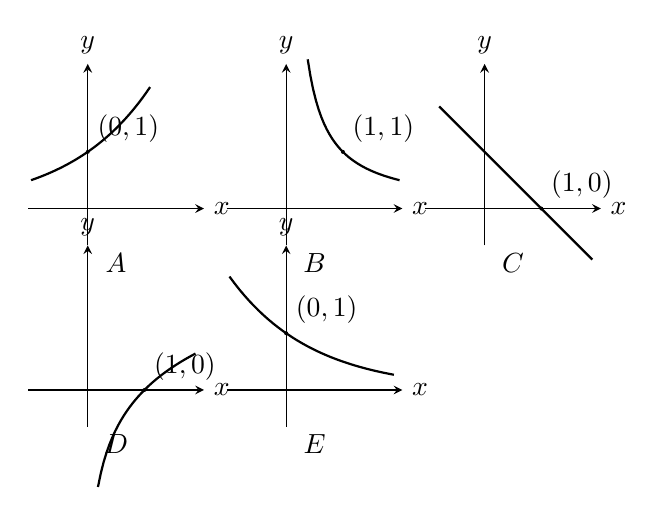
\begin{tikzpicture}[scale=0.72,>=stealth]
  \foreach \x/\y/\label in {0/0/A,3.5/0/B,7/0/C,0/-3.2/D,3.5/-3.2/E} {
    \begin{scope}[shift={(\x,\y)}]
      \draw[->] (-1.05,0)--(2.05,0) node[right] {$x$};
      \draw[->] (0,-0.65)--(0,2.55) node[above] {$y$};
      \node[below] at (0.5,-0.62) {$\label$};
    \end{scope}
  }
  % A：递增指数曲线，过 (0,1)
  \begin{scope}
    \draw[thick,domain=-1:1.1,samples=35] plot (\x,{2^\x});
    \fill (0,1) circle (1pt) node[above right] {$(0,1)$};
  \end{scope}
  % B：仅第一象限递减，标点 (1,1)
  \begin{scope}[shift={(3.5,0)}]
    \draw[thick,domain=0.38:2,samples=35] plot (\x,{1/\x});
    \fill (1,1) circle (1pt) node[above right] {$(1,1)$};
  \end{scope}
  % C：递减并穿过 (1,0)
  \begin{scope}[shift={(7,0)}]
    \draw[thick,domain=-0.8:1.9,samples=35] plot (\x,{1-\x});
    \fill (1,0) circle (1pt) node[above right] {$(1,0)$};
  \end{scope}
  % D：递增对数形曲线，过 (1,0)
  \begin{scope}[shift={(0,-3.2)}]
    \draw[thick,domain=0.18:1.9,samples=35] plot (\x,{ln(\x)});
    \fill (1,0) circle (1pt) node[above right] {$(1,0)$};
  \end{scope}
  % E：递减指数曲线，过 (0,1)，向右趋近 x 轴
  \begin{scope}[shift={(3.5,-3.2)}]
    \draw[thick,domain=-1:1.9,samples=35] plot (\x,{2^(-\x)});
    \fill (0,1) circle (1pt) node[above right] {$(0,1)$};
  \end{scope}
\end{tikzpicture}
